\documentclass[aspectratio=169]{beamer}
\title{Improvements and current status of the ACTS-based ITk main pass reconstruction}
\author{Andreas Stefl, Noemi Calace, Paul Gessinger-Befurt, Carlo Varni, Pierfrancesco Butti}
\institute{CERN}
\date{2025-08-18}

\setbeamertemplate{navigation symbols}{}

\begin{document}

\frame{\titlepage}

\begin{frame}
\frametitle{Pixel clustering}
\begin{figure}[h]
    \centering
    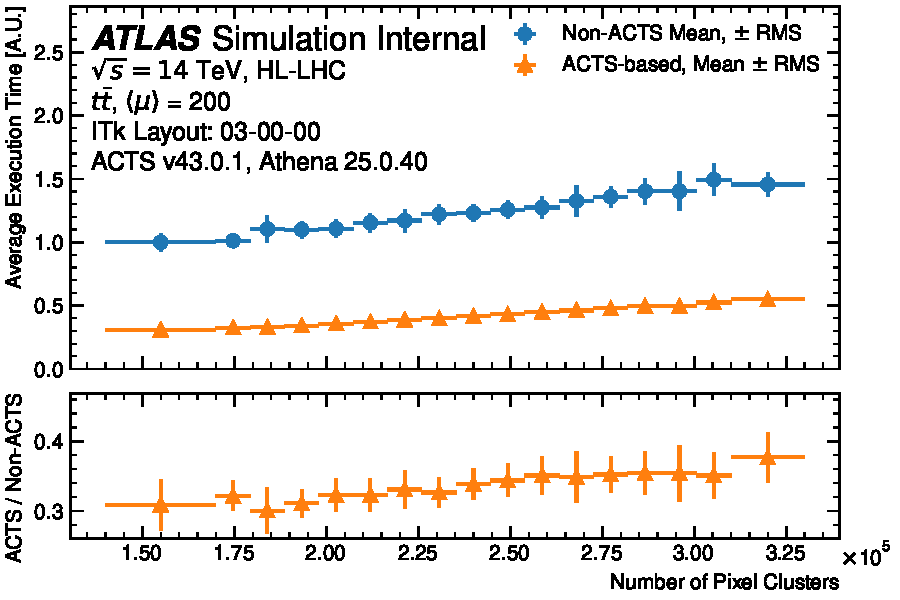
\includegraphics[width=0.4\textwidth]{plots/clustering_pixel.pdf}
    \caption{Average execution time (in arbitrary units) of the pixel clustering algorithms as a function of the number of reconstructed pixel clusters, obtained with the Athena framework running the current implementation of the clustering algorithm (comparable to the one used during Run 3 operations) and a modified version including the ACTS toolkit. The measurement was taken on the same machine and the same set of $t\bar{t}$ events at $\langle \mu \rangle = 200$ with a center of mass energy of $\sqrt{s}=14$ TeV, using the ITk Layout 03-00-00. An average timing improvement per event of $\sim3\times$ with the ACTS based clustering algorithm is observed while achieving exactly identical physics results.}
\end{figure}
\end{frame}

\begin{frame}
\frametitle{Strip clustering}
\begin{figure}[h]
    \centering
    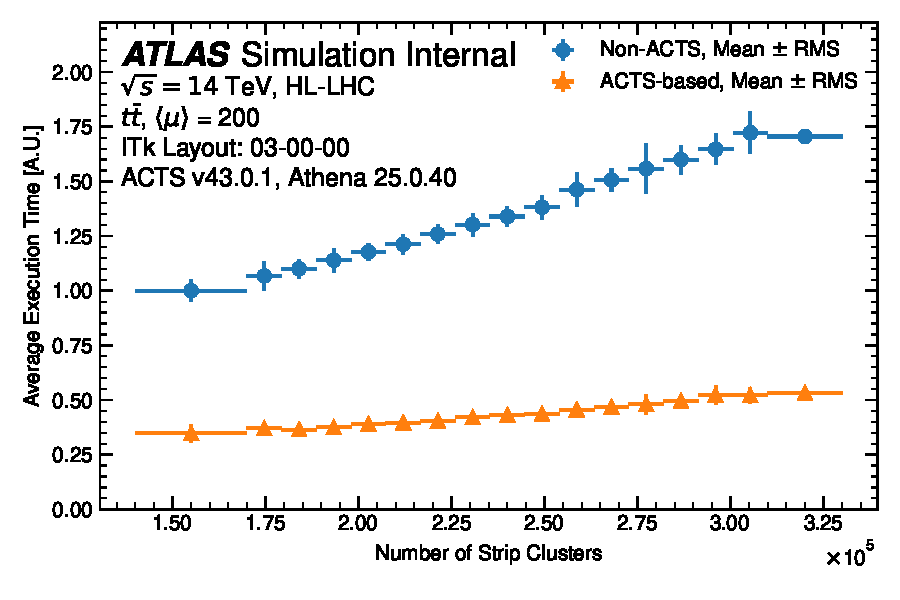
\includegraphics[width=0.4\textwidth]{plots/clustering_strip.pdf}
    \caption{Average execution time (in arbitrary units) of the strip clustering algorithms as a function of the number of reconstructed strip clusters, obtained with the Athena framework running the current implementation of the clustering algorithm (comparable to the one used during Run 3 operations) and a modified version including the ACTS toolkit. The measurement was taken on the same machine and the same set of $t\bar{t}$ events at $\langle \mu \rangle = 200$ with a center of mass energy of $\sqrt{s}=14$ TeV, using the ITk Layout 03-00-00. An average timing improvement per event of $\sim3\times$ with the ACTS based clustering algorithm is observed while achieving exactly identical physics results.}
\end{figure}
\end{frame}

% \begin{frame}
% \frametitle{Pixel seeding}
% \begin{figure}[h]
%     \centering
%     \includegraphics[width=0.7\textwidth]{plots/seeding_pixel.pdf}
%     \caption{}
%     \label{fig:seeding_pixel}
% \end{figure}
% \end{frame}

\begin{frame}
\frametitle{Tracking efficiency}
\begin{figure}[h]
    \centering
    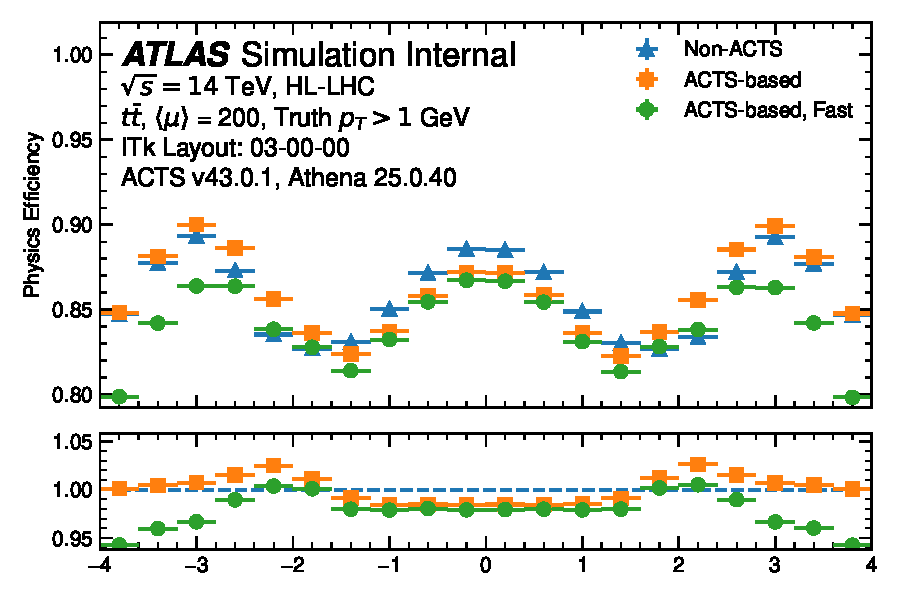
\includegraphics[width=0.4\textwidth]{plots/tracking_efficiency_physics.pdf}
    \caption{Tracking efficiency as a function of the pseudo-rapidity $\eta$ of the associated truth particle using the ITk Layout 03-00-00 for $t\bar{t}$ events at $\langle \mu \rangle = 200$. Efficiency is defined as the ratio between the number of reconstructed tracks matched to truth particle and all selected truth particles. The truth particles considered must satisfy $p_\mathrm{T} > 1$ GeV and $|\eta| < 4.0$, and be produced by the primary interactions and are matched to a reconstructed track if the matching probability is larger than 50\%. Track candidates are reconstructed using the ACTS Combinatorial Kalman Filter from ACTS v43.0.1 in Athena 25.0.40. Final tracks are fulfilling the following list of requirements: number of measurements (pixel + strip) $\geq 7$, $p_\mathrm{T}^\mathrm{reco} > 900$ MeV (400 MeV) in $|\eta| < 2.0$ ($2.0 < |\eta| < 4.0$), $|z_0^\mathrm{reco}| \leq 20$ cm and $|d_0^\mathrm{reco}| \leq 2$ mm (10 mm) in $|\eta| < 2.6$ ($2.6 < |\eta| < 4.0$).}
\end{figure}
\end{frame}

\begin{frame}
\frametitle{Tracking resolution $\sigma(d_0)$}
\begin{figure}[h]
    \centering
    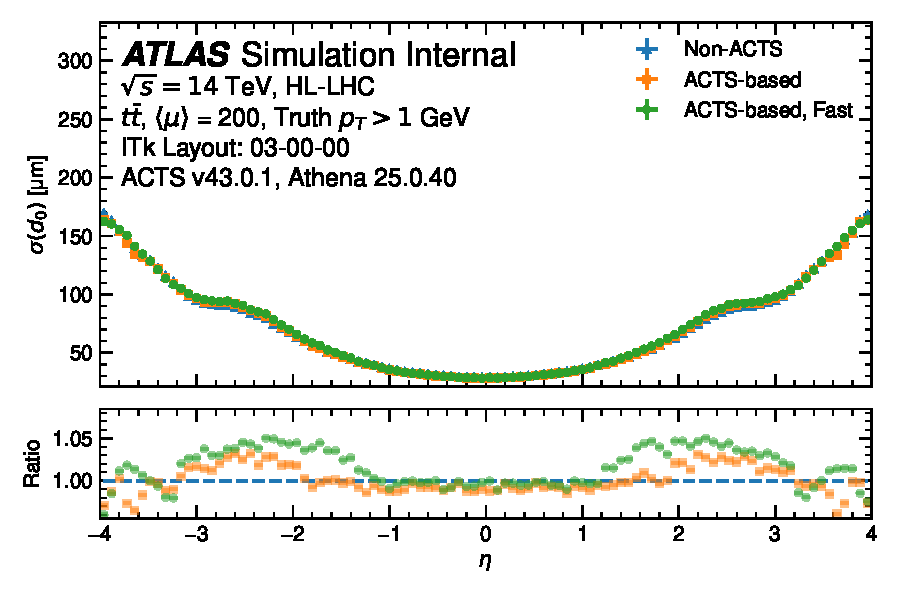
\includegraphics[width=0.7\textwidth]{plots/tracking_resolution_d0.pdf}
    \caption{}
\end{figure}
\end{frame}

\begin{frame}
\frametitle{Tracking resolution $\sigma(z_0)$}
\begin{figure}[h]
    \centering
    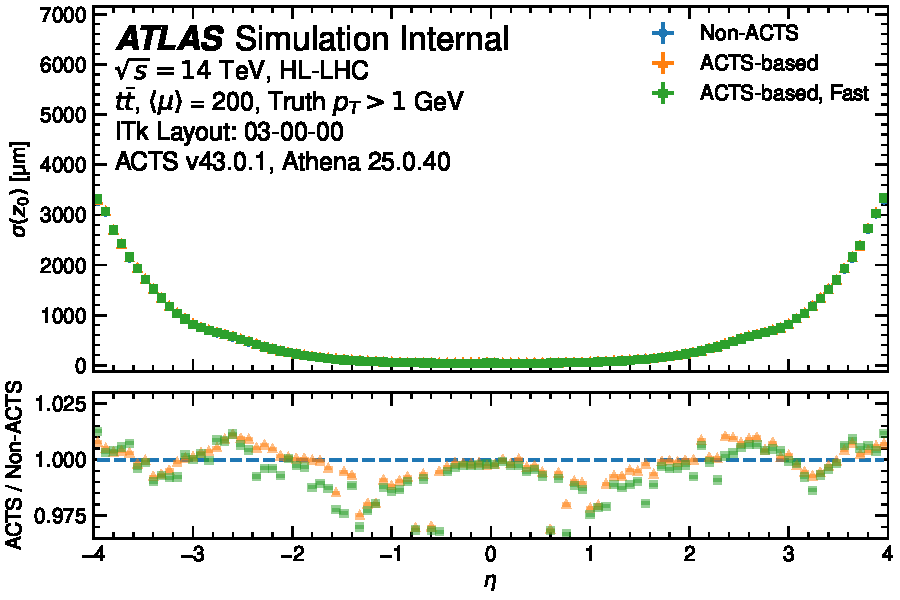
\includegraphics[width=0.7\textwidth]{plots/tracking_resolution_z0.pdf}
    \caption{}
\end{figure}
\end{frame}

\begin{frame}
\frametitle{Tracking resolution $p_t \ \sigma(q/p_t)$}
\begin{figure}[h]
    \centering
    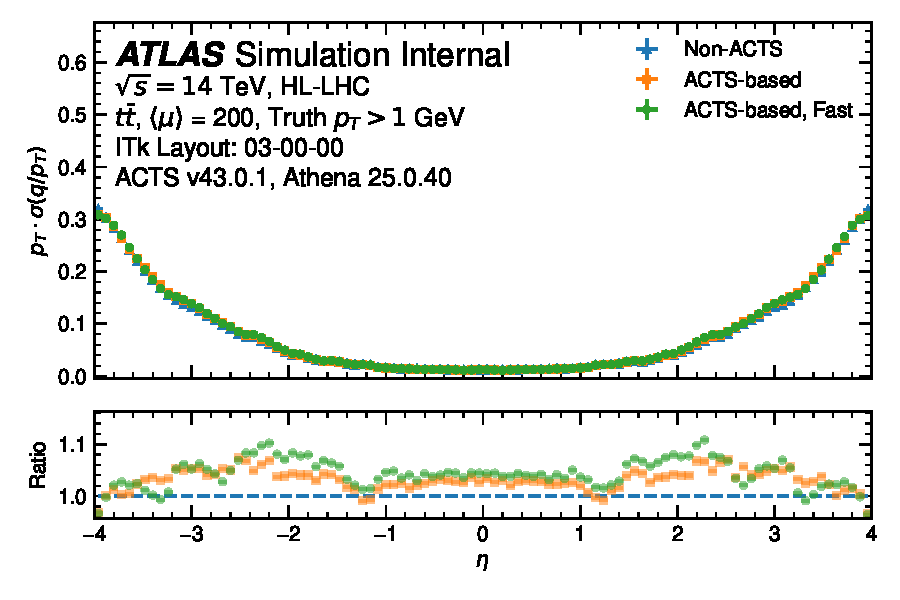
\includegraphics[width=0.7\textwidth]{plots/tracking_resolution_ptqopt.pdf}
    \caption{}
\end{figure}
\end{frame}

\begin{frame}
\frametitle{CPU time evolution}
\begin{figure}[h]
    \centering
    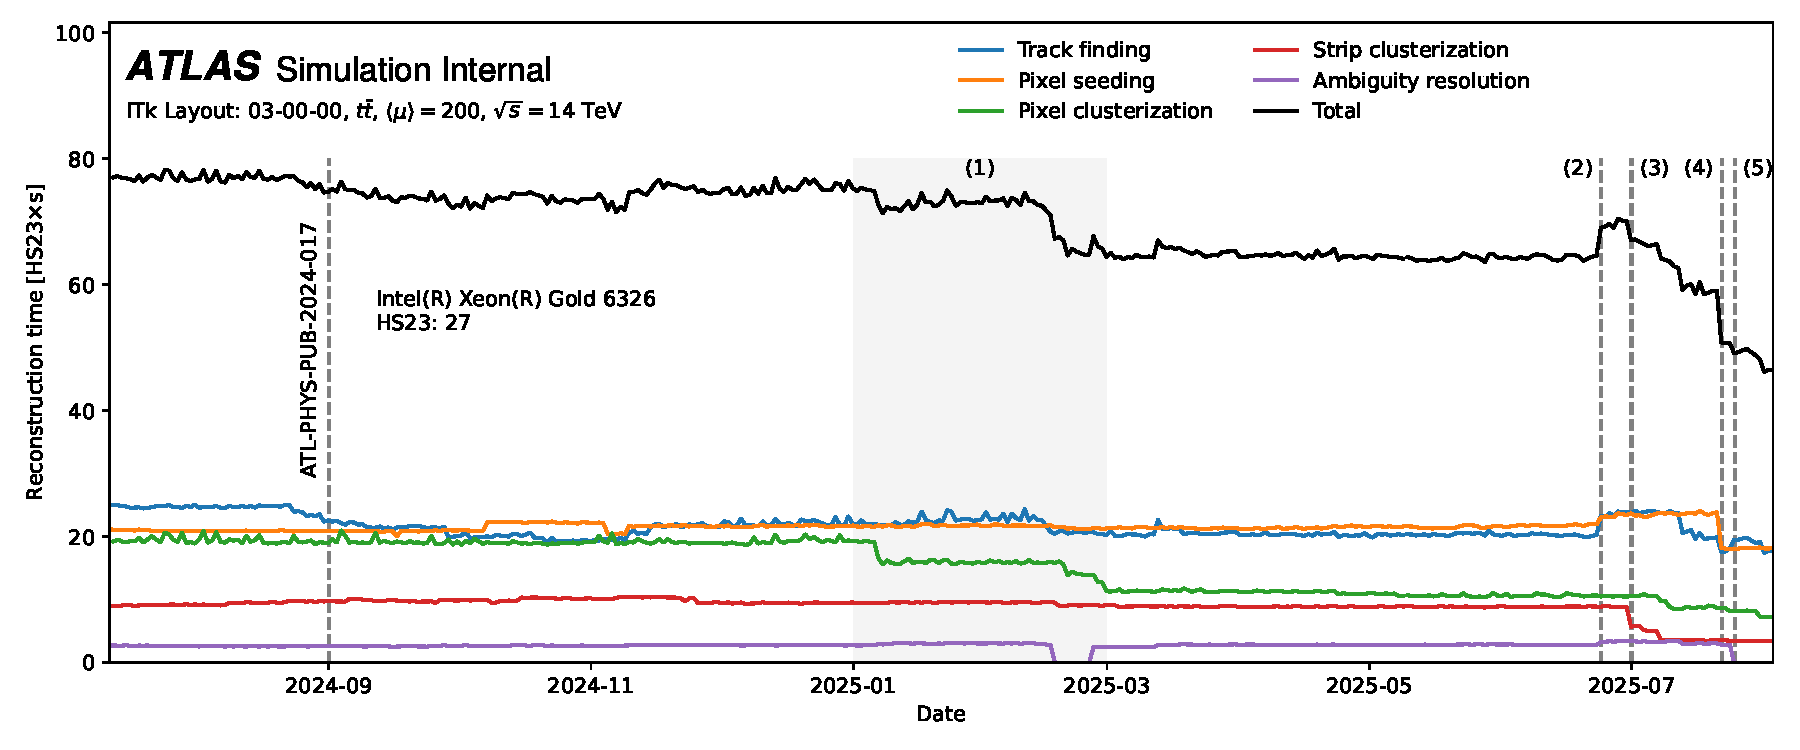
\includegraphics[width=1.0\textwidth]{plots/spot.pdf}
    \caption{}
\end{figure}
\end{frame}

\end{document}
